\documentclass{beamer}

\mode<presentation>
{
  \usetheme{ANLBlue}
  \setbeamercovered{transparent=20}
}

\usepackage[english]{babel}
\usepackage[latin1]{inputenc}
\usepackage{alltt,listings,multirow,ulem,siunitx}
\usepackage[absolute,overlay]{textpos}
\TPGrid{1}{1}
\usepackage{pdfpages}
\usepackage{ulem}
\usepackage{multimedia}
\usepackage{multicol}
\newcommand\hmmax{0}
\newcommand\bmmax{0}
\usepackage{bm}
\usepackage{comment}
\usepackage{subcaption}

% font definitions, try \usepackage{ae} instead of the following
% three lines if you don't like this look
\usepackage{mathptmx}
\usepackage[scaled=.90]{helvet}
% \usepackage{courier}
\usepackage[T1]{fontenc}
\usepackage{tikz}
\usetikzlibrary{decorations.pathreplacing}
\usetikzlibrary{shadows,arrows,shapes.misc,shapes.arrows,shapes.multipart,arrows,decorations.pathmorphing,backgrounds,positioning,fit,petri,calc,shadows,chains,matrix}

\usepackage{JedMacros}

\title{How can we quantify \\ performance versatility?}
\author{{\bf Jed Brown} \texttt{jedbrown@mcs.anl.gov} (ANL and CU Boulder)}

% Real applications are often constrained by factors such as external
% requirements for time-to-solution, a need to fit within some level of
% memory, or to accommodate workflow demands involving human decisions,
% provenance, proprietary software, or the like.  Consequently, the region
% of multi-dimensional configuration space that an application cares about
% may be disjoint from the single point or path chosen by authors when
% promoting their new algorithm or machine.  Different authors are likely
% to choose different configurations, leading to results that are not very
% useful to applications.  Drawing on experience and performance data
% obtained while developing the HPGMG benchmark (https://hpgmg.org) and
% working with PETSc applications, we discuss issues and methods for
% collecting and presenting performance data to express versatility and
% improve relevance to applications.

% - Use the \inst command only if there are several affiliations.
% - Keep it simple, no one is interested in your street address.
% \institute
% {
%   Mathematics and Computer Science Division \\ Argonne National Laboratory
% }

\date{JointLab, Chicago, 2014-11-24 \\[1em]
{\small This talk: \url{http://59A2.org/files/20141124-Versatility.pdf}}}

% This is only inserted into the PDF information catalog. Can be left
% out.
\subject{Talks}


% If you have a file called "university-logo-filename.xxx", where xxx
% is a graphic format that can be processed by latex or pdflatex,
% resp., then you can add a logo as follows:

% \pgfdeclareimage[height=0.5cm]{university-logo}{university-logo-filename}
% \logo{\pgfuseimage{university-logo}}



% Delete this, if you do not want the table of contents to pop up at
% the beginning of each subsection:
% \AtBeginSubsection[]
% {
% \begin{frame}<beamer>
%   \frametitle{Outline}
%   \tableofcontents[currentsection,currentsubsection]
% \end{frame}
% }

% \AtBeginSection[]
% {
%   \begin{frame}<beamer>
%     \frametitle{Outline}
%     \tableofcontents[currentsection]
%   \end{frame}
% }

% If you wish to uncover everything in a step-wise fashion, uncomment
% the following command:

% \beamerdefaultoverlayspecification{<+->}

\begin{document}
\lstset{language=C}
\normalem

\begin{frame}{Exascale Science \& Engineering Demands}
  \begin{itemize}
  \item Model fidelity: resolution, multi-scale, coupling
    \begin{itemize}
    \item Transient simulation is not weak scaling: $\Delta t \sim \Delta x$
    \end{itemize}
  \item Analysis using a sequence of forward simulations
    \begin{itemize}
    \item Inversion, data assimilation, optimization
    \item Quantify uncertainty, risk-aware decisions
    \end{itemize}
  \item Increasing relevance $\implies$ external requirements on time
    \begin{itemize}
    \item Policy: 5 SYPD to inform IPCC
    \item Weather, manufacturing, field studies, disaster response
    \end{itemize}
  \item ``weak scaling'' [\ldots] will increasingly give way to ``strong scaling''\\
    {\scriptsize [The International Exascale Software Project Roadmap, 2011]}
  \item ACME @ \SI{15}{\kilo\metre} scaling saturates at $<10\%$ of Titan (CPU) or Mira
    \begin{itemize}
    \item Cannot decrease $\Delta x$: SYPD would be too slow to calibrate
    \item ``results'' would be meaningless for 50-100y predictions, a ``stunt run''
    \end{itemize}
  \item \alert{\bf ACME v1 goal of 5 SYPD is pure strong scaling.}
    \begin{itemize}
    \item Many non-climate applications in same position.
    \end{itemize}
  \end{itemize}
\end{frame}

\begin{frame}{HPGMG-FE on Edison, SuperMUC, Titan}
  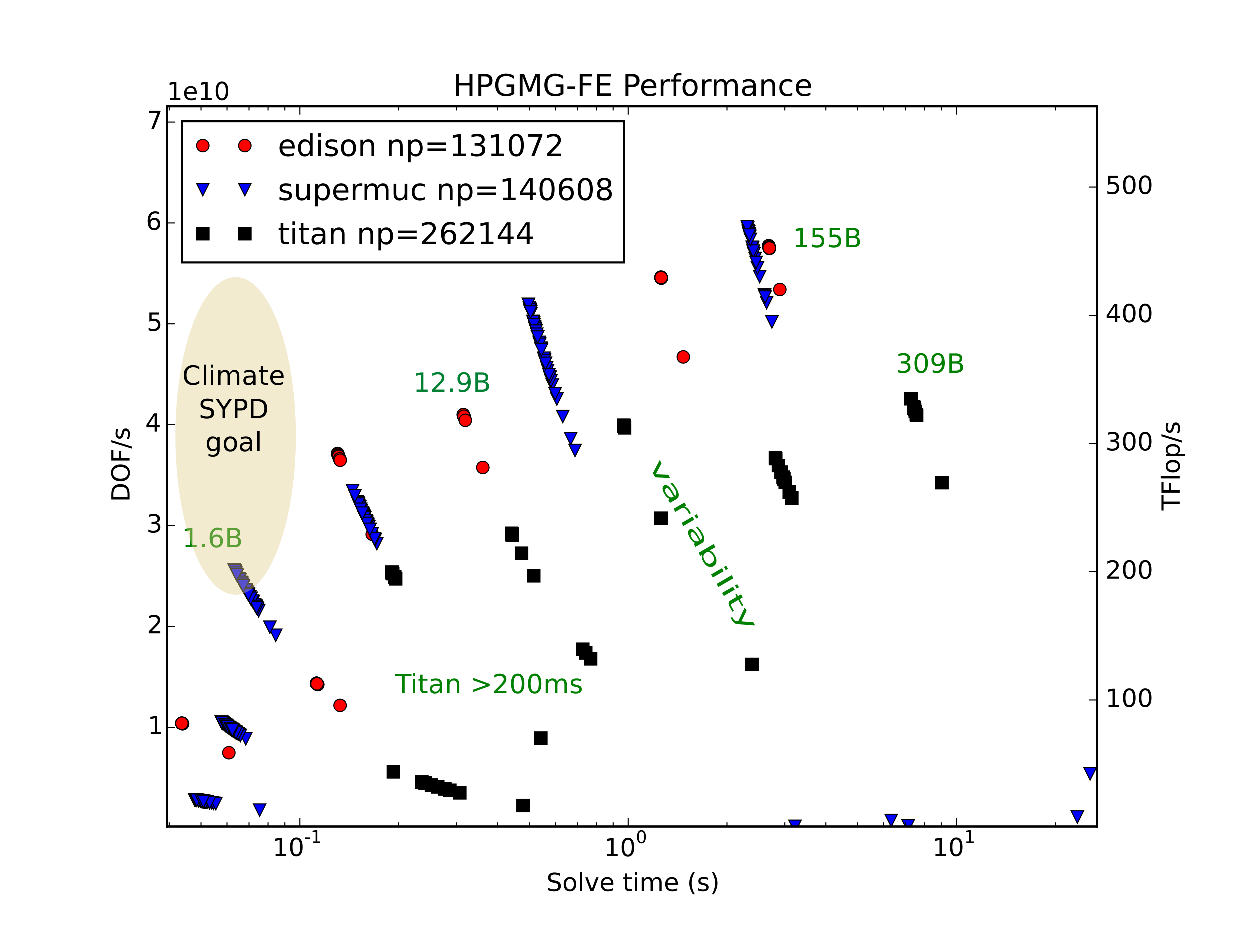
\includegraphics[width=\textwidth]{figures/hpgmg/range-edison-supermuc-titan-ann2.eps}
\end{frame}

\begin{frame}{ASCR Exascale Hardware Roadmap}
  \begin{itemize}
  \item Finer-grained parallelism
    \begin{itemize}
    \item Larger number of simple, slow cores
    \item Longer vector units, more hardware threads
    \end{itemize}
  \item On-node synchronization costs increasing
    \begin{itemize}
    \item \texttt{omp parallel} is more than 20k cycles on KNC
    \item 10x more than network messaging latency, like \texttt{MPI\_Allreduce} on 1M cores of BG/Q
    \end{itemize}
  \item L1 cache sizes stagnant, smaller slices per way of parallelism
  \item Stagnant DRAM bandwidth, narrow HBM ``sweet spot''
    \begin{itemize}
    \item DDR4 channels cheaper (Watt and \$) on 2014 HSW than 2016 KNL
    \end{itemize}
  \item Improved network bandwidth, latency stagnant
  \item Coprocessors increase latency (kernel launch, network)
  \item \alert{\bf Nothing to improve strong scaling.}
    \begin{itemize}
    \item Hardware changes orthogonal to improving ACME SYPD
    \item Enables larger ensembles, not higher resolution
    \item Tim Palmer's call for \SI{1}{\kilo\metre} requires different approach to hardware
    \end{itemize}
  \end{itemize}
\end{frame}

\end{document}
